\documentclass{standalone}
\usepackage{tikz}
\usetikzlibrary{patterns, positioning}


\begin{document}
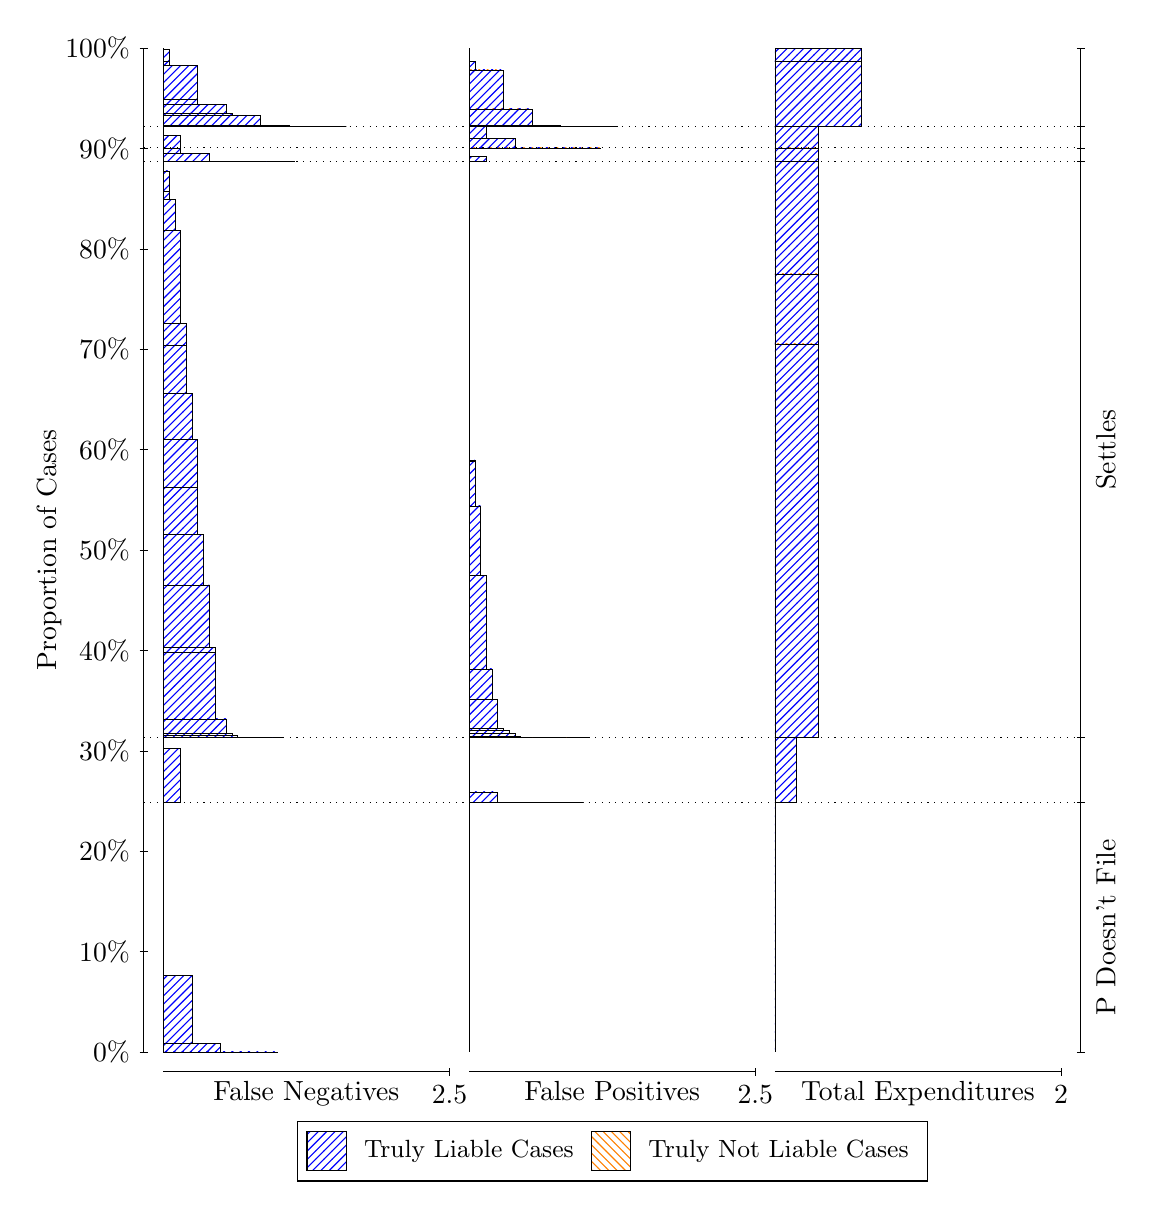
\begin{tikzpicture}
\draw[black, very thin] (1.5,1.75) -- (1.5,14.5);
\node[rotate=90, text=black, anchor=center] at (0.3, 8.125) {Proportion of Cases};
\draw[black, very thin] (1.45,1.75) -- (1.55,1.75);
\node[text=black, anchor=east] at (1.45, 1.75) {0\%};
\draw[black, very thin] (1.45,3.025) -- (1.55,3.025);
\node[text=black, anchor=east] at (1.45, 3.025) {10\%};
\draw[black, very thin] (1.45,4.3) -- (1.55,4.3);
\node[text=black, anchor=east] at (1.45, 4.3) {20\%};
\draw[black, very thin] (1.45,5.575) -- (1.55,5.575);
\node[text=black, anchor=east] at (1.45, 5.575) {30\%};
\draw[black, very thin] (1.45,6.85) -- (1.55,6.85);
\node[text=black, anchor=east] at (1.45, 6.85) {40\%};
\draw[black, very thin] (1.45,8.125) -- (1.55,8.125);
\node[text=black, anchor=east] at (1.45, 8.125) {50\%};
\draw[black, very thin] (1.45,9.4) -- (1.55,9.4);
\node[text=black, anchor=east] at (1.45, 9.4) {60\%};
\draw[black, very thin] (1.45,10.675) -- (1.55,10.675);
\node[text=black, anchor=east] at (1.45, 10.675) {70\%};
\draw[black, very thin] (1.45,11.95) -- (1.55,11.95);
\node[text=black, anchor=east] at (1.45, 11.95) {80\%};
\draw[black, very thin] (1.45,13.225) -- (1.55,13.225);
\node[text=black, anchor=east] at (1.45, 13.225) {90\%};
\draw[black, very thin] (1.45,14.5) -- (1.55,14.5);
\node[text=black, anchor=east] at (1.45, 14.5) {100\%};

\draw[black, very thin] (13.4,1.75) -- (13.4,14.5);
\draw[black, very thin] (13.35,1.75) -- (13.45,1.75);
\node[anchor=west] at (13.35, 1.75) {};
\draw[black, very thin] (13.35,4.9192) -- (13.45,4.9192);
\node[anchor=west] at (13.35, 4.9192) {};
\draw[black, very thin] (13.35,5.7439) -- (13.45,5.7439);
\node[anchor=west] at (13.35, 5.7439) {};
\draw[black, very thin] (13.35,13.057) -- (13.45,13.057);
\node[anchor=west] at (13.35, 13.057) {};
\draw[black, very thin] (13.35,13.232) -- (13.45,13.232);
\node[anchor=west] at (13.35, 13.232) {};
\draw[black, very thin] (13.35,13.504) -- (13.45,13.504);
\node[anchor=west] at (13.35, 13.504) {};
\draw[black, very thin] (13.35,14.5) -- (13.45,14.5);
\node[anchor=west] at (13.35, 14.5) {};

\draw[black, very thin, pattern color=blue, pattern=north east lines] (1.75,1.75) rectangle (3.2033,1.75);
\draw[black, very thin, pattern color=blue, pattern=north east lines] (1.75,1.75) rectangle (2.84,1.7509);
\draw[black, very thin, pattern color=blue, pattern=north east lines] (1.75,1.7509) rectangle (2.4767,1.8606);
\draw[black, very thin, pattern color=blue, pattern=north east lines] (1.75,1.8606) rectangle (2.1133,2.7238);
\draw[black, very thin, pattern color=orange, pattern=north west lines] (1.75,2.7238) rectangle (1.75,2.7238);
\draw[black, very thin, pattern color=blue, pattern=north east lines] (1.75,2.7238) rectangle (1.75,4.9192);
\draw[black, very thin, pattern color=blue, pattern=north east lines] (1.75,4.9192) rectangle (1.968,5.6089);
\draw[black, very thin, pattern color=orange, pattern=north west lines] (1.75,5.6089) rectangle (1.75,5.6089);
\draw[black, very thin, pattern color=blue, pattern=north east lines] (1.75,5.6089) rectangle (1.75,5.7439);
\draw[black, very thin, pattern color=blue, pattern=north east lines] (1.75,5.7439) rectangle (3.276,5.7439);
\draw[black, very thin, pattern color=blue, pattern=north east lines] (1.75,5.7439) rectangle (3.1307,5.7439);
\draw[black, very thin, pattern color=blue, pattern=north east lines] (1.75,5.7439) rectangle (2.9853,5.7439);
\draw[black, very thin, pattern color=blue, pattern=north east lines] (1.75,5.7439) rectangle (2.9127,5.7439);
\draw[black, very thin, pattern color=blue, pattern=north east lines] (1.75,5.7439) rectangle (2.84,5.7439);
\draw[black, very thin, pattern color=blue, pattern=north east lines] (1.75,5.7439) rectangle (2.7673,5.744);
\draw[black, very thin, pattern color=blue, pattern=north east lines] (1.75,5.744) rectangle (2.6947,5.7743);
\draw[black, very thin, pattern color=blue, pattern=north east lines] (1.75,5.7743) rectangle (2.622,5.7963);
\draw[black, very thin, pattern color=blue, pattern=north east lines] (1.75,5.7963) rectangle (2.5493,5.9806);
\draw[black, very thin, pattern color=blue, pattern=north east lines] (1.75,5.9806) rectangle (2.4767,5.9816);
\draw[black, very thin, pattern color=blue, pattern=north east lines] (1.75,5.9816) rectangle (2.404,6.8274);
\draw[black, very thin, pattern color=blue, pattern=north east lines] (1.75,6.8274) rectangle (2.404,6.8845);
\draw[black, very thin, pattern color=blue, pattern=north east lines] (1.75,6.8845) rectangle (2.3313,7.6827);
\draw[black, very thin, pattern color=blue, pattern=north east lines] (1.75,7.6827) rectangle (2.2587,8.3205);
\draw[black, very thin, pattern color=blue, pattern=north east lines] (1.75,8.3205) rectangle (2.186,8.9218);
\draw[black, very thin, pattern color=blue, pattern=north east lines] (1.75,8.9218) rectangle (2.186,9.531);
\draw[black, very thin, pattern color=blue, pattern=north east lines] (1.75,9.531) rectangle (2.1133,10.116);
\draw[black, very thin, pattern color=blue, pattern=north east lines] (1.75,10.116) rectangle (2.0407,10.731);
\draw[black, very thin, pattern color=blue, pattern=north east lines] (1.75,10.731) rectangle (2.0407,10.999);
\draw[black, very thin, pattern color=blue, pattern=north east lines] (1.75,10.999) rectangle (1.968,12.186);
\draw[black, very thin, pattern color=blue, pattern=north east lines] (1.75,12.186) rectangle (1.8953,12.573);
\draw[black, very thin, pattern color=blue, pattern=north east lines] (1.75,12.573) rectangle (1.8227,12.686);
\draw[black, very thin, pattern color=blue, pattern=north east lines] (1.75,12.686) rectangle (1.8227,12.94);
\draw[black, very thin, pattern color=blue, pattern=north east lines] (1.75,12.94) rectangle (1.75,12.941);
\draw[black, very thin, pattern color=orange, pattern=north west lines] (1.75,12.941) rectangle (1.75,12.941);
\draw[black, very thin, pattern color=blue, pattern=north east lines] (1.75,12.941) rectangle (1.75,13.057);
\draw[black, very thin, pattern color=blue, pattern=north east lines] (1.75,13.057) rectangle (3.4213,13.057);
\draw[black, very thin, pattern color=blue, pattern=north east lines] (1.75,13.057) rectangle (3.058,13.057);
\draw[black, very thin, pattern color=blue, pattern=north east lines] (1.75,13.057) rectangle (2.6947,13.06);
\draw[black, very thin, pattern color=blue, pattern=north east lines] (1.75,13.06) rectangle (2.3313,13.163);
\draw[black, very thin, pattern color=blue, pattern=north east lines] (1.75,13.163) rectangle (1.968,13.232);
\draw[black, very thin, pattern color=orange, pattern=north west lines] (1.75,13.232) rectangle (1.75,13.232);
\draw[black, very thin, pattern color=blue, pattern=north east lines] (1.75,13.232) rectangle (1.968,13.386);
\draw[black, very thin, pattern color=orange, pattern=north west lines] (1.75,13.386) rectangle (1.75,13.386);
\draw[black, very thin, pattern color=blue, pattern=north east lines] (1.75,13.386) rectangle (1.75,13.504);
\draw[black, very thin, pattern color=blue, pattern=north east lines] (1.75,13.504) rectangle (4.0753,13.504);
\draw[black, very thin, pattern color=blue, pattern=north east lines] (1.75,13.504) rectangle (3.712,13.504);
\draw[black, very thin, pattern color=blue, pattern=north east lines] (1.75,13.504) rectangle (3.3487,13.521);
\draw[black, very thin, pattern color=blue, pattern=north east lines] (1.75,13.521) rectangle (3.276,13.521);
\draw[black, very thin, pattern color=blue, pattern=north east lines] (1.75,13.521) rectangle (2.9853,13.649);
\draw[black, very thin, pattern color=blue, pattern=north east lines] (1.75,13.649) rectangle (2.9127,13.649);
\draw[black, very thin, pattern color=blue, pattern=north east lines] (1.75,13.649) rectangle (2.622,13.669);
\draw[black, very thin, pattern color=blue, pattern=north east lines] (1.75,13.669) rectangle (2.5493,13.781);
\draw[black, very thin, pattern color=blue, pattern=north east lines] (1.75,13.781) rectangle (2.2587,13.781);
\draw[black, very thin, pattern color=blue, pattern=north east lines] (1.75,13.781) rectangle (2.186,13.852);
\draw[black, very thin, pattern color=blue, pattern=north east lines] (1.75,13.852) rectangle (2.186,14.278);
\draw[black, very thin, pattern color=blue, pattern=north east lines] (1.75,14.278) rectangle (1.8953,14.278);
\draw[black, very thin, pattern color=blue, pattern=north east lines] (1.75,14.278) rectangle (1.8227,14.334);
\draw[black, very thin, pattern color=blue, pattern=north east lines] (1.75,14.334) rectangle (1.8227,14.485);
\draw[black, very thin, pattern color=orange, pattern=north west lines] (1.75,14.485) rectangle (1.75,14.485);
\draw[black, very thin, pattern color=blue, pattern=north east lines] (1.75,14.485) rectangle (1.75,14.5);
\draw[black, very thin, pattern color=orange, pattern=north west lines] (5.6333,1.75) rectangle (5.6333,1.75);
\draw[black, very thin, pattern color=blue, pattern=north east lines] (5.6333,1.75) rectangle (5.6333,4.9192);
\draw[black, very thin, pattern color=orange, pattern=north west lines] (5.6333,4.9192) rectangle (7.0867,4.9192);
\draw[black, very thin, pattern color=blue, pattern=north east lines] (5.6333,4.9192) rectangle (7.0867,4.9192);
\draw[black, very thin, pattern color=blue, pattern=north east lines] (5.6333,4.9192) rectangle (6.7233,4.9192);
\draw[black, very thin, pattern color=blue, pattern=north east lines] (5.6333,4.9192) rectangle (6.36,4.9203);
\draw[black, very thin, pattern color=blue, pattern=north east lines] (5.6333,4.9203) rectangle (5.9967,5.0542);
\draw[black, very thin, pattern color=blue, pattern=north east lines] (5.6333,5.0542) rectangle (5.6333,5.7439);
\draw[black, very thin, pattern color=orange, pattern=north west lines] (5.6333,5.7439) rectangle (7.1593,5.7439);
\draw[black, very thin, pattern color=blue, pattern=north east lines] (5.6333,5.7439) rectangle (7.1593,5.7439);
\draw[black, very thin, pattern color=orange, pattern=north west lines] (5.6333,5.7439) rectangle (6.8687,5.7439);
\draw[black, very thin, pattern color=blue, pattern=north east lines] (5.6333,5.7439) rectangle (6.8687,5.7439);
\draw[black, very thin, pattern color=blue, pattern=north east lines] (5.6333,5.7439) rectangle (6.796,5.7439);
\draw[black, very thin, pattern color=orange, pattern=north west lines] (5.6333,5.7439) rectangle (6.7233,5.7439);
\draw[black, very thin, pattern color=blue, pattern=north east lines] (5.6333,5.7439) rectangle (6.7233,5.7439);
\draw[black, very thin, pattern color=orange, pattern=north west lines] (5.6333,5.7439) rectangle (6.578,5.7439);
\draw[black, very thin, pattern color=blue, pattern=north east lines] (5.6333,5.7439) rectangle (6.578,5.7439);
\draw[black, very thin, pattern color=blue, pattern=north east lines] (5.6333,5.7439) rectangle (6.5053,5.7439);
\draw[black, very thin, pattern color=blue, pattern=north east lines] (5.6333,5.7439) rectangle (6.4327,5.7439);
\draw[black, very thin, pattern color=orange, pattern=north west lines] (5.6333,5.7439) rectangle (6.4327,5.7439);
\draw[black, very thin, pattern color=blue, pattern=north east lines] (5.6333,5.7439) rectangle (6.4327,5.7439);
\draw[black, very thin, pattern color=blue, pattern=north east lines] (5.6333,5.7439) rectangle (6.36,5.7441);
\draw[black, very thin, pattern color=orange, pattern=north west lines] (5.6333,5.7441) rectangle (6.2873,5.7441);
\draw[black, very thin, pattern color=blue, pattern=north east lines] (5.6333,5.7441) rectangle (6.2873,5.7554);
\draw[black, very thin, pattern color=blue, pattern=north east lines] (5.6333,5.7554) rectangle (6.2147,5.7987);
\draw[black, very thin, pattern color=orange, pattern=north west lines] (5.6333,5.7987) rectangle (6.142,5.7987);
\draw[black, very thin, pattern color=blue, pattern=north east lines] (5.6333,5.7987) rectangle (6.142,5.8374);
\draw[black, very thin, pattern color=blue, pattern=north east lines] (5.6333,5.8374) rectangle (6.0693,5.8599);
\draw[black, very thin, pattern color=blue, pattern=north east lines] (5.6333,5.8599) rectangle (6.0693,5.8608);
\draw[black, very thin, pattern color=orange, pattern=north west lines] (5.6333,5.8608) rectangle (5.9967,5.8608);
\draw[black, very thin, pattern color=blue, pattern=north east lines] (5.6333,5.8608) rectangle (5.9967,6.2275);
\draw[black, very thin, pattern color=blue, pattern=north east lines] (5.6333,6.2275) rectangle (5.924,6.6141);
\draw[black, very thin, pattern color=blue, pattern=north east lines] (5.6333,6.6141) rectangle (5.8513,7.8015);
\draw[black, very thin, pattern color=blue, pattern=north east lines] (5.6333,7.8015) rectangle (5.7787,8.6845);
\draw[black, very thin, pattern color=blue, pattern=north east lines] (5.6333,8.6845) rectangle (5.706,9.2462);
\draw[black, very thin, pattern color=blue, pattern=north east lines] (5.6333,9.2462) rectangle (5.706,9.2694);
\draw[black, very thin, pattern color=blue, pattern=north east lines] (5.6333,9.2694) rectangle (5.6333,13.057);
\draw[black, very thin, pattern color=orange, pattern=north west lines] (5.6333,13.057) rectangle (5.8513,13.057);
\draw[black, very thin, pattern color=blue, pattern=north east lines] (5.6333,13.057) rectangle (5.8513,13.126);
\draw[black, very thin, pattern color=blue, pattern=north east lines] (5.6333,13.126) rectangle (5.6333,13.232);
\draw[black, very thin, pattern color=orange, pattern=north west lines] (5.6333,13.232) rectangle (7.3047,13.232);
\draw[black, very thin, pattern color=blue, pattern=north east lines] (5.6333,13.232) rectangle (7.3047,13.232);
\draw[black, very thin, pattern color=blue, pattern=north east lines] (5.6333,13.232) rectangle (6.9413,13.232);
\draw[black, very thin, pattern color=blue, pattern=north east lines] (5.6333,13.232) rectangle (6.578,13.232);
\draw[black, very thin, pattern color=blue, pattern=north east lines] (5.6333,13.232) rectangle (6.2147,13.349);
\draw[black, very thin, pattern color=blue, pattern=north east lines] (5.6333,13.349) rectangle (5.8513,13.504);
\draw[black, very thin, pattern color=orange, pattern=north west lines] (5.6333,13.504) rectangle (7.5227,13.504);
\draw[black, very thin, pattern color=blue, pattern=north east lines] (5.6333,13.504) rectangle (7.5227,13.504);
\draw[black, very thin, pattern color=orange, pattern=north west lines] (5.6333,13.504) rectangle (7.1593,13.504);
\draw[black, very thin, pattern color=blue, pattern=north east lines] (5.6333,13.504) rectangle (7.1593,13.504);
\draw[black, very thin, pattern color=orange, pattern=north west lines] (5.6333,13.504) rectangle (6.796,13.504);
\draw[black, very thin, pattern color=blue, pattern=north east lines] (5.6333,13.504) rectangle (6.796,13.518);
\draw[black, very thin, pattern color=orange, pattern=north west lines] (5.6333,13.518) rectangle (6.4327,13.518);
\draw[black, very thin, pattern color=blue, pattern=north east lines] (5.6333,13.518) rectangle (6.4327,13.726);
\draw[black, very thin, pattern color=orange, pattern=north west lines] (5.6333,13.726) rectangle (6.36,13.726);
\draw[black, very thin, pattern color=blue, pattern=north east lines] (5.6333,13.726) rectangle (6.36,13.726);
\draw[black, very thin, pattern color=blue, pattern=north east lines] (5.6333,13.726) rectangle (6.0693,14.223);
\draw[black, very thin, pattern color=orange, pattern=north west lines] (5.6333,14.223) rectangle (5.9967,14.223);
\draw[black, very thin, pattern color=blue, pattern=north east lines] (5.6333,14.223) rectangle (5.9967,14.223);
\draw[black, very thin, pattern color=blue, pattern=north east lines] (5.6333,14.223) rectangle (5.706,14.334);
\draw[black, very thin, pattern color=orange, pattern=north west lines] (5.6333,14.334) rectangle (5.6333,14.334);
\draw[black, very thin, pattern color=blue, pattern=north east lines] (5.6333,14.334) rectangle (5.6333,14.5);
\draw[black, very thin, pattern color=orange, pattern=north west lines] (9.5167,1.75) rectangle (9.5167,1.75);
\draw[black, very thin, pattern color=blue, pattern=north east lines] (9.5167,1.75) rectangle (9.5167,4.9192);
\draw[black, very thin, pattern color=orange, pattern=north west lines] (9.5167,4.9192) rectangle (9.7892,4.9192);
\draw[black, very thin, pattern color=blue, pattern=north east lines] (9.5167,4.9192) rectangle (9.7892,5.7439);
\draw[black, very thin, pattern color=orange, pattern=north west lines] (9.5167,5.7439) rectangle (10.062,5.7439);
\draw[black, very thin, pattern color=blue, pattern=north east lines] (9.5167,5.7439) rectangle (10.062,10.744);
\draw[black, very thin, pattern color=orange, pattern=north west lines] (9.5167,10.744) rectangle (10.062,10.744);
\draw[black, very thin, pattern color=blue, pattern=north east lines] (9.5167,10.744) rectangle (10.062,11.631);
\draw[black, very thin, pattern color=orange, pattern=north west lines] (9.5167,11.631) rectangle (10.062,11.631);
\draw[black, very thin, pattern color=blue, pattern=north east lines] (9.5167,11.631) rectangle (10.062,13.057);
\draw[black, very thin, pattern color=orange, pattern=north west lines] (9.5167,13.057) rectangle (10.062,13.057);
\draw[black, very thin, pattern color=blue, pattern=north east lines] (9.5167,13.057) rectangle (10.062,13.232);
\draw[black, very thin, pattern color=orange, pattern=north west lines] (9.5167,13.232) rectangle (10.062,13.232);
\draw[black, very thin, pattern color=blue, pattern=north east lines] (9.5167,13.232) rectangle (10.062,13.504);
\draw[black, very thin, pattern color=orange, pattern=north west lines] (9.5167,13.504) rectangle (10.607,13.504);
\draw[black, very thin, pattern color=blue, pattern=north east lines] (9.5167,13.504) rectangle (10.607,14.334);
\draw[black, very thin, pattern color=orange, pattern=north west lines] (9.5167,14.334) rectangle (10.607,14.334);
\draw[black, very thin, pattern color=blue, pattern=north east lines] (9.5167,14.334) rectangle (10.607,14.5);
\draw[black, dotted] (1.5,4.9192) -- (13.4,4.9192);
\draw[black, dotted] (1.5,5.7439) -- (13.4,5.7439);
\draw[black, dotted] (1.5,13.057) -- (13.4,13.057);
\draw[black, dotted] (1.5,13.232) -- (13.4,13.232);
\draw[black, dotted] (1.5,13.504) -- (13.4,13.504);
\draw[black, very thin] (1.75,1.5) -- (5.3833,1.5);
\node[text=black, anchor=north] at (3.5667, 1.5) {False Negatives};
\draw[black, very thin] (5.3833,1.45) -- (5.3833,1.55);
\node[text=black, anchor=north] at (5.3833, 1.45) {2.5};

\draw[black, very thin] (5.6333,1.5) -- (9.2667,1.5);
\node[text=black, anchor=north] at (7.45, 1.5) {False Positives};
\draw[black, very thin] (9.2667,1.45) -- (9.2667,1.55);
\node[text=black, anchor=north] at (9.2667, 1.45) {2.5};

\draw[black, very thin] (9.5167,1.5) -- (13.15,1.5);
\node[text=black, anchor=north] at (11.333, 1.5) {Total Expenditures};
\draw[black, very thin] (13.15,1.45) -- (13.15,1.55);
\node[text=black, anchor=north] at (13.15, 1.45) {2};

\node[text=black, centered, rotate=90] at (13.72, 3.3346) {P Doesn't File};

\node[text=black, centered, rotate=90] at (13.72, 9.4002) {Settles};




\draw (7.449999999999999,1.5) node[draw=none] (baseCoordinate) {};
\begin{scope}[align=center]
        \matrix[scale=0.5, draw=black, below=0.5cm of baseCoordinate, nodes={draw}, column sep=0.1cm]{
            \node[rectangle, draw, minimum width=0.5cm, minimum height=0.5cm, pattern color=blue, pattern=north east lines] {}; &
            \node[draw=none, font=\small, text=black] (B) {Truly Liable Cases}; &
            \node[rectangle, draw, minimum width=0.5cm, minimum height=0.5cm, pattern color=orange, pattern=north west lines] {}; &
            \node[draw=none, font=\small, text=black] (B) {Truly Not Liable Cases}; \\
            };
\end{scope}

\end{tikzpicture}
\end{document}